\documentclass[letterpaper,10pt]{book}
% Change to 10 pt
\usepackage{pdfpages}
\usepackage{morewrites}			% to counteract the no write space problem
\setcounter{tocdepth}{6}

\usepackage[framemethod=TikZ]{mdframed}

\usepackage{fancyhdr}

\usepackage{paralist}
\usepackage{amsmath}
\usepackage{amsfonts}
\usepackage{amssymb}
\usepackage{graphicx}

\usepackage{datetime}
%\usepackage{ulem}

%\usepackage[nottoc]{toobibind}

\usepackage[inline]{enumitem}

% Outer margin at 2.50 is exacty correct to fit the ``corruption alert'' tables
\usepackage[inner=1.0in, outer=2.50in, top=2.54cm,bottom=2.54cm, marginparwidth=2.25in]{geometry}

\usepackage{marginnote}
\usepackage{longtable}
\usepackage{booktabs}
\usepackage{xcolor}

\usepackage{soul}

%%%%%%%%%%%%
\definecolor{ForestGreen}{rgb}{0.00,0.29,0.098}
%%%%%%%%%%%%

\usepackage{marginnote}

\usepackage{imakeidx} 
\usepackage[
	backref=true,
	style=numeric,
%	citestyle=numeric,
	backend=bibtex
	]{biblatex}
\usepackage[driverfallback=hypertex,colorlinks=True]{hyperref}
\usepackage{cleveref}

\makeindex[name=scripture,columnsep=20pt, columnseprule=True,columns=3, title=Scripture References]
\makeindex[name=speaker,columnsep=20pt, columnseprule=True,,columns=2, title=Sermon Creator]
\makeindex[name=series,columnsep=20pt, columnseprule=True,,columns=2, title=Sermon Series]
\makeindex[name=date,columnsep=20pt, columnseprule=True,columns=2, title=Sermon Date]
\makeindex[name=event,columnsep=20pt, columnseprule=True,columns=2, title=Event]
\makeindex[name=topic,columnsep=20pt, columnseprule=True,columns=2, title=Topic]
\makeindex[name=AWIP,columnsep=20pt, columnseprule=True,columns=3, title=All Words in Passage]
\makeindex[name=NWIV,columnsep=20pt, columnseprule=True,columns=3, title=Number of Words in Verse]
\makeindex[name=PNIP,columnsep=20pt, columnseprule=True,columns=3, title=Proper Names in Passage]
\makeindex[name=PEIP,columnsep=20pt, columnseprule=True,columns=2, title=Prophetic Events in Passage]
\makeindex[name=TWPAQ,columnsep=20pt, columnseprule=True,columns=1, title=13-Word Phrases and Quotes]
\makeindex[name=PFTTIS,columnsep=20pt, columnseprule=False,columns=3, title=Phrases found 13 times in scripture]
\makeindex[name=WFTTIS,columnsep=20pt, columnseprule=False,columns=3, title=Words found 13 times in scripture]
\makeindex[name=WFITV,columnsep=20pt, columnseprule=False,columns=3, title=Words found in exactly 13 verses]
\makeindex[name=EVENTS,columnsep=20pt, columnseprule=False,columns=2, title=Sermon Log by Place]
\makeindex[name=QUESTIONS,columnsep=20pt, columnseprule=False,columns=2, title=Bible Questions]
\makeindex[name=DOCTRINES,columnsep=20pt, columnseprule=False,columns=2, title=Doctrines]
\makeindex[name=SONGS,columnsep=20pt, columnseprule=False,columns=1, title=Songs]
\makeindex[name=LOCATION,columnsep=20pt, columnseprule=False,columns= 2, title=Location]
\makeindex[name=FACEBOOK,columnsep=20pt, columnseprule=False,columns=2, title=Facebook]
\makeindex[name=DEVOTIONAL,columnsep=20pt, columnseprule=False,columns=2, title=Devotional Items]
%%%%%%%%%%%%%%%%% EXTRA COLORS
\definecolor{champagne}{rgb}{0.97,0.91,0.81}
\definecolor{bone}{rgb}{0.89,0.85,0.79}
\pagestyle{fancy}
\fancyhf{}
\fancyhead[LE,RO]{\today}
\fancyhead[RE,LO]{Daily Bible Reading}
\fancyhead[CE,CO]{-page \thepage  - }

\fancyfoot[CO,CE]{\leftmark}
%\fancyfoot[LE,RO]{CSCE 692, HW1}

\title{DBR\\
Daily \\ Reads}
\author{Keith Anthony \\
\today }
%+/ffffff +   \pagenumbering{gobble}
\bibliography{Bibliographies/All20220122}

\setlength{\fboxsep}{1.0pt}

\usepackage[utf8]{inputenc}
\usepackage{tikz}

\begin{document}
%%%%%%%%%%%% Tile Page

\begin{titlepage}

\begin{flushright}
\rightskip=-2.5cm
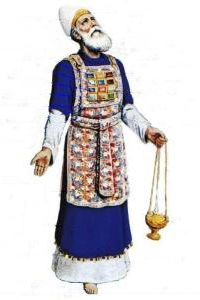
\includegraphics[width=50mm,scale=1.5]{Extras/Melchisedec.jpg}
\vspace{0.4in}  % Create a title for the document and write it in bold font
\LARGE{\textbf{\date}} % Again, do a line break
\linebreak 
% Create a subtitle \large{with Outlines, Statistics, Cross References, and Notes}
\vspace{0.5in}
\begin{flushleft}
\LARGE{Day \#70: Friday, 11 March 2022 PLAIN  \\}\vspace{0.25in}
\LARGE{Joshua 16-18 Psalm 70 Proverb 11}
\end{flushleft}
\vspace{0.6in}
\bigskip

\normalsize{Xenia, Oh.\\}
\normalsize{created: \today}
\vspace{1.3in}

\end{flushright}
\end{titlepage}

\newpage 
\tableofcontents\hypertarget{TOC}{}
\listoffigures
\listoftables

\hyphenation{A-bim-e-lech bre-thren E-phra-im  Gib-e-o-nites Jer-u-sa-lem through-out Phil-i-stines The-o-phil-us Am-a-le-kites ven-geance Mesh-el-e-mi-ah onan-ism Phar-a-oh thoughts grev-ous-ness Hach-a-liah adul-ter-er Shad-rach}

%%%%%%%%%%%%%%%%% EXTRA COLORS
%%%%%%%%%%%%%%%%% EXTRA COLORS
%%%%%%%%%%%%%%%%% EXTRA COLORS
\definecolor{champagne}{rgb}{0.97,0.91,0.81}
\definecolor{bone}{rgb}{0.89,0.85,0.79}

\definecolor{ForestGreen}{rgb}{0.00,0.29,0.098}
\definecolor{GIVING}{cmyk}{1,0.0,0.72,.1}

\definecolor{MLPE}{cmyk}{1,1,0,.45}
\definecolor{SOCCER}{cmyk}{.77, 0, .42, .49}
\definecolor{PAYBILL}{cmyk}{0,0.83,0.76,0.07}
\definecolor{SERMON}{cmyk}{.14,.9,0,.30} % aka seance \href{http://www.flatuicolorpicker.com/purple-cmyk-color-model/}{seance}
\definecolor{BIBLE}{cmyk}{0,.17,.74,.17}
\definecolor{WORKBLUE}{cmyk}{1, .5, 0, .6}
\definecolor{myOrange}{cmyk}{0, .4, .98, .03}
\definecolor{myTan}{cmyk}{0.0,.07,.17,.10}
\definecolor{myRed}{cmyk}{0,1,1,0}
\definecolor{myWhite}{cmyk}{0,0,0,0}
\definecolor{BLUESoD}{cmyk}{.97,.84,0,.04}
\definecolor{WHITE}{cmyk}{0,0,0,0}
\definecolor{OLDGOLD}{cmyk}{0.05,0.3,1.00,0}
\definecolor{CASTLETON}{cmyk}{1,0,0.31,0.66}
\definecolor{cadmiumgreen}{rgb}{0.0, 0.42, 0.24}
\definecolor{jungle}{rgb}{0.203,0.4882,0.1718}
\definecolor{MYGOLD}{rgb}{1,.84,0}

\definecolor{MYLIGHTGRAY}{rgb}{.85,.85,.85}

\definecolor{codegreen}{rgb}{0,0.6,0}
\definecolor{codegray}{rgb}{0.5,0.5,0.5}
\definecolor{codepurple}{rgb}{0.58,0,0.82}
\definecolor{backcolour}{rgb}{0.95,0.95,0.92}


\mdfdefinestyle{MyFrame}{%
    linecolor=blue,
    outerlinewidth=2pt,
    roundcorner=5pt,
    innertopmargin=\baselineskip,
    innerbottommargin=\baselineskip,
    innerrightmargin=10pt,
    innerleftmargin=10pt,
    backgroundcolor=gray!25!white}


\mdfdefinestyle{MyFrame2}{%
    linecolor=black,
    outerlinewidth=2pt,
    roundcorner=5pt,
    innertopmargin=\baselineskip,
    innerbottommargin=\baselineskip,
    innerrightmargin=10pt,
    innerleftmargin=10pt,
    backgroundcolor=yellow!25!white}


%%%%%
%% for PFTTIS list
%%%%%

%%% And Joseph said unto
\index[PFTTIS]{And Joseph said unto!Genesis!Gen 40:008}
\index[PFTTIS]{And Joseph said unto!Genesis!Gen 40:012}
\index[PFTTIS]{And Joseph said unto!Genesis!Gen 41:025}
\index[PFTTIS]{And Joseph said unto!Genesis!Gen 42:014}
\index[PFTTIS]{And Joseph said unto!Genesis!Gen 42:018}
\index[PFTTIS]{And Joseph said unto!Genesis!Gen 44:015}
\index[PFTTIS]{And Joseph said unto!Genesis!Gen 45:003}
\index[PFTTIS]{And Joseph said unto!Genesis!Gen 45:004}
\index[PFTTIS]{And Joseph said unto!Genesis!Gen 46:031}
\index[PFTTIS]{And Joseph said unto!Genesis!Gen 48:009}
\index[PFTTIS]{And Joseph said unto!Genesis!Gen 48:018}
\index[PFTTIS]{And Joseph said unto!Genesis!Gen 50:019}
\index[PFTTIS]{And Joseph said unto!Genesis!Gen 50:024}


%%% a shadow
\index[PFTTIS]{a shadow!1Chronicles!1Chr 029:15}
\index[PFTTIS]{a shadow!Job!Job 008:09}
\index[PFTTIS]{a shadow!Job!Job 014:02}
\index[PFTTIS]{a shadow!Job!Job 017:07}
\index[PFTTIS]{a shadow!Psalm!Psa 102:011}
\index[PFTTIS]{a shadow!Psalm!Psa 144:004}
\index[PFTTIS]{a shadow!Ecclesiastes!Eccl 006:012}
\index[PFTTIS]{a shadow!Ecclesiastes!Eccl 008:013}
\index[PFTTIS]{a shadow!Isaiah!Isa 04:006}
\index[PFTTIS]{a shadow!Isaiah!Isa 25:004}
\index[PFTTIS]{a shadow!Jonah!Jnh 04:06}
\index[PFTTIS]{a shadow!Colossians!Col 02:017}
\index[PFTTIS]{a shadow!Hebews!Heb 10:001}

%%% blessed is the man
\index[PFTTIS]{blessed is the man!Psalm!Psa 001:001}
\index[PFTTIS]{blessed is the man!Psalm!Psa 032:002}
\index[PFTTIS]{blessed is the man!Psalm!Psa 034:008}
\index[PFTTIS]{blessed is the man!Psalm!Psa 065:004}
\index[PFTTIS]{blessed is the man!Psalm!Psa 084:005}
\index[PFTTIS]{blessed is the man!Psalm!Psa 084:012}
\index[PFTTIS]{blessed is the man!Psalm!Psa 094:012}
\index[PFTTIS]{blessed is the man!Psalm!Psa 112:001}
\index[PFTTIS]{blessed is the man!Proverbs!Pro 008:034}
\index[PFTTIS]{blessed is the man!Isaiah!Isa 056:002}
\index[PFTTIS]{blessed is the man!Jeremiah!Jer 017:007}
\index[PFTTIS]{blessed is the man!Romans!Rom 004:008}
\index[PFTTIS]{blessed is the man!James!Jam 001:012}


%%% carry them
\index[PFTTIS]{carry them!Leviticus!Lev 14:045}
\index[PFTTIS]{carry them!Numbers!Num 11:012}
\index[PFTTIS]{carry them!Joshua!Jsh 04:003}
\index[PFTTIS]{carry them!1Samuel!1Sam 20:040}
\index[PFTTIS]{carry them!1Kings!1Kng 08:046}
\index[PFTTIS]{carry them!2Chronicles!2Chr 06:036}
\index[PFTTIS]{carry them!Ezra!Ezra 05:015}
\index[PFTTIS]{carry them!Isaiah!Isa 40:011}
\index[PFTTIS]{carry them!Isaiah!Isa 41:016}
\index[PFTTIS]{carry them!Isaiah!Isa 57:013}
\index[PFTTIS]{carry them!Jeremiah!Jer 20:004}
\index[PFTTIS]{carry them!Jeremiah!Jer 20:005}
\index[PFTTIS]{carry them!Jeremiah!Jer 43:012}


\index[PFTTIS]{good tidings!2Samuel!2Sam 18:027}
\index[PFTTIS]{good tidings!1Kings!1Ki 01:042}
\index[PFTTIS]{good tidings!2Kings!2Ki 07:009 (2x)}
\index[PFTTIS]{good tidings!Isaiah!Isa 40:009 (2x)}
\index[PFTTIS]{good tidings!Isaiah!Isa 41:007}
\index[PFTTIS]{good tidings!Isaiah!Isa 52:007}
\index[PFTTIS]{good tidings!Isaiah!Isa 61:001}
\index[PFTTIS]{good tidings!Nahum!Nah 01:005}
\index[PFTTIS]{good tidings!Luke!Lk 02:010}
\index[PFTTIS]{good tidings!1Thessalonians!1Thess 03:006}


%%% dead body
\index[PFTTIS]{dead body!Leviticus!Lev 21:011}
\index[PFTTIS]{dead body!Numbers!Num 06:006}
\index[PFTTIS]{dead body!Numbers!Num 09:006}
\index[PFTTIS]{dead body!Numbers!Num 09:007}
\index[PFTTIS]{dead body!Numbers!Num 09:010}
\index[PFTTIS]{dead body!Numbers!Num 09:011}
\index[PFTTIS]{dead body!Numbers!Num 09:013}
\index[PFTTIS]{dead body!Numbers!Num 09:016}
\index[PFTTIS]{dead body!2Kings!2Ki 08:005}
\index[PFTTIS]{dead body!Isaiah!Isa 26:019}
\index[PFTTIS]{dead body!Jeremiah!Jer 26:023}
\index[PFTTIS]{dead body!Jeremiah!Jer 36:030}
\index[PFTTIS]{dead body!Haggai!Hag 02:013}

%%% great sea
\index[PFTTIS]{great sea!Numbers!Num 34:006}
\index[PFTTIS]{great sea!Numbers!Num 34:007}
\index[PFTTIS]{great sea!Joshua!Jos 01:004}
\index[PFTTIS]{great sea!Joshua!Jos 09:001}
\index[PFTTIS]{great sea!Joshua!Jos 15:012}
\index[PFTTIS]{great sea!Joshua!Jos 15:047}
\index[PFTTIS]{great sea!Joshua!Jos 23:004}
\index[PFTTIS]{great sea!Ezekiel!Eze 47:010}
\index[PFTTIS]{great sea!Ezekiel!Eze 47:015}
\index[PFTTIS]{great sea!Ezekiel!Eze 47:019}
\index[PFTTIS]{great sea!Ezekiel!Eze 47:020}
\index[PFTTIS]{great sea!Ezekiel!Eze 48:028}
\index[PFTTIS]{great sea!Daniel!Dan 07:002}


%%% have forsaken me
\index[PFTTIS]{have forsaken me!Judges!Jdg 10:013}
\index[PFTTIS]{have forsaken me!1Samuel!1Sam 08:008}
\index[PFTTIS]{have forsaken me!1Kings!1Ki 11:033}
\index[PFTTIS]{have forsaken me!2Kings!2Ki 22:017}
\index[PFTTIS]{have forsaken me!2Chronicles!2Chr 12:005}
\index[PFTTIS]{have forsaken me!2Chronicles!2Chr 34:025}
\index[PFTTIS]{have forsaken me!Jeremiah!Jer 01:016}
\index[PFTTIS]{have forsaken me!Jeremiah!Jer 02:013}
\index[PFTTIS]{have forsaken me!Jeremiah!Jer 05:007}
\index[PFTTIS]{have forsaken me!Jeremiah!Jer 05:019}
\index[PFTTIS]{have forsaken me!Jeremiah!Jer 16:011 (2x)}
\index[PFTTIS]{have forsaken me!Jeremiah!Jer 19:004}

%%% no king
\index[PFTTIS]{no king!Judges!Jdg 17:06}
\index[PFTTIS]{no king!Judges!Jdg 18:01}
\index[PFTTIS]{no king!Judges!Jdg 19:01}
\index[PFTTIS]{no king!Judges!Jdg 21:25}
\index[PFTTIS]{no king!1Kings!1Ki 22:47}
\index[PFTTIS]{no king!2Kings!2Ki 23:25}
\index[PFTTIS]{no king!Nehemiah!Neh 13:26}
\index[PFTTIS]{no king!Psalms!Psa 033:016}
\index[PFTTIS]{no king!Proverbs!Pro 30:27}
\index[PFTTIS]{no king!Daniel!Dan 02:10}
\index[PFTTIS]{no king!Hosea!Hos 10:03}
\index[PFTTIS]{no king!Micah!Mic 04:09}
\index[PFTTIS]{no king!John!Jhn 19:15}


%%% rebellious house
\index[PFTTIS]{rebellious house!Exodus!Exo 02:005}
\index[PFTTIS]{rebellious house!Exodus!Exo 02:006}
\index[PFTTIS]{rebellious house!Exodus!Exo 02:008}
\index[PFTTIS]{rebellious house!Exodus!Exo 03:009}
\index[PFTTIS]{rebellious house!Exodus!Exo 03:026}
\index[PFTTIS]{rebellious house!Exodus!Exo 03:027}
\index[PFTTIS]{rebellious house!Exodus!Exo 12:002 (2x)}
\index[PFTTIS]{rebellious house!Exodus!Exo 12:003}
\index[PFTTIS]{rebellious house!Exodus!Exo 12:009}
\index[PFTTIS]{rebellious house!Exodus!Exo 12:025}
\index[PFTTIS]{rebellious house!Exodus!Exo 17:012}
\index[PFTTIS]{rebellious house!Exodus!Exo 24:003}

%%% seek him
\index[PFTTIS]{seek him!Deuteronomy!Deu 04:029}\index[PFTTIS]{seek him!1Samuel!1Sam 23:025}
\index[PFTTIS]{seek him!1Chronicles!1Chr 28:009}
\index[PFTTIS]{seek him!2Chronicles!1Chr 15:002}
\index[PFTTIS]{seek him!Ezra!Ezr 08:022}
\index[PFTTIS]{seek him!Psalms!Psa 022:026}
\index[PFTTIS]{seek him!Psalms!Psa 024:006}
\index[PFTTIS]{seek him!Psalms!Psa 119:002}
\index[PFTTIS]{seek him!SoS!SoS 03:002}
\index[PFTTIS]{seek him!SoS!SoS 06:001}
\index[PFTTIS]{seek him!Hosea!Hos 07:010}
\index[PFTTIS]{seek him!Amos!Amo 05:008}
\index[PFTTIS]{seek him!Hebrews!Heb 11:0063}


%%% seek ye
\index[PFTTIS]{seek ye!Isaiah!Isa 34:016}
\index[PFTTIS]{seek ye!Isaiah!Isa 45:019}
\index[PFTTIS]{seek ye!Isaiah!Isa 55:006}
\index[PFTTIS]{seek ye!Amos!Amos 5:004}
\index[PFTTIS]{seek ye!John!John 1:38}
\index[PFTTIS]{seek ye!John!John 18:4}
\index[PFTTIS]{seek ye!John!John 18:7}
\index[PFTTIS]{seek ye!Matthew!Matt 6:33}
\index[PFTTIS]{seek ye!Numbers!Num 16:10}
\index[PFTTIS]{seek ye!Luke!Luke 12:31}
\index[PFTTIS]{seek ye!Luke!Luke 24:5}
\index[PFTTIS]{seek ye!Psalm!Psa 27:8}
\index[PFTTIS]{seek ye!Zephaniah!Zeph 2:3}

%%% the uncircumcised
\index[PFTTIS]{the uncircumcised!Genesis!Gen 17:014}
\index[PFTTIS]{the uncircumcised!Judges!Jdg 14:003}
\index[PFTTIS]{the uncircumcised!Judges!Jdg 15:018}
\index[PFTTIS]{the uncircumcised!2Samuel!2Sam 01:020}
\index[PFTTIS]{the uncircumcised!Isaiah!Isa 02:001}
\index[PFTTIS]{the uncircumcised!Jeremiah!Jer 09:025}
\index[PFTTIS]{the uncircumcised!Ezekiel!Eze 28:010}
\index[PFTTIS]{the uncircumcised!Ezekiel!Eze 31:018}
\index[PFTTIS]{the uncircumcised!Ezekiel!Eze 32:019}
\index[PFTTIS]{the uncircumcised!Ezekiel!Eze 32:027}
\index[PFTTIS]{the uncircumcised!Ezekiel!Eze 32:028}
\index[PFTTIS]{the uncircumcised!Ezekiel!Eze 32:029}
\index[PFTTIS]{the uncircumcised!Ezekiel!Eze 32:032}

%%% worship him
\index[PFTTIS]{worship him!Psalms!Psa 97:007}
\index[PFTTIS]{worship him!Zephaniah!Zeph 02:011}
\index[PFTTIS]{worship him!Matthew!Matt 02:002}
\index[PFTTIS]{worship him!Matthew!Matt 02:008}
\index[PFTTIS]{worship him!John!John 04:023}
\index[PFTTIS]{worship him!John!John 04:024 (2x)} 
\index[PFTTIS]{worship him!Acts!Acts 17:023}
\index[PFTTIS]{worship him!Hebrews!Heb 01:006}
\index[PFTTIS]{worship him!Revelation!Rev 04:010}
\index[PFTTIS]{worship him!Revelation!Rev 13:008}
\index[PFTTIS]{worship him!Revelation!Rev 14:007}
\index[PFTTIS]{worship him!Revelation!Rev 19:010}


%%%%%
%% for PFTTIS list
%%%%%

%%% afflictions
\index[WFTTIS]{afflictions!Psalms!Psa 34:019}
\index[WFTTIS]{afflictions!Psalms!Psa 132:001}
\index[WFTTIS]{afflictions!Acts!Acts 07:010}
\index[WFTTIS]{afflictions!Acts!Acts 20:023}
\index[WFTTIS]{afflictions!2Corinthians!2Cor 06:004}
\index[WFTTIS]{afflictions!Colossians!Col 01:024}
\index[WFTTIS]{afflictions!1Thessalonians!1Thess 03:003}
\index[WFTTIS]{afflictions!2Timothy!2Tim 01:008}
\index[WFTTIS]{afflictions!2Timothy!2Tim 03:011}
\index[WFTTIS]{afflictions!2Timothy!2Tim 04:005}
\index[WFTTIS]{afflictions!Hebrews!Heb 10:032}
\index[WFTTIS]{afflictions!Hebrews!Heb 10:033}
\index[WFTTIS]{afflictions!1Peter!1Pet 05:009}

%%% acsend
\index[WFTTIS]{acsend!Joshua!Jos 06:05}
\index[WFTTIS]{acsend!Psalm!Psa 024:003}
\index[WFTTIS]{acsend!Psalm!Psa 135:007}
\index[WFTTIS]{acsend!Psalm!Psa 139:008}
\index[WFTTIS]{acsend!Isaiah!Isa 14:013}
\index[WFTTIS]{acsend!Isaiah!Isa 14:014}
\index[WFTTIS]{acsend!Jeremiah!Jer 10:013}
\index[WFTTIS]{acsend!Jeremiah!Jer 51:016}
\index[WFTTIS]{acsend!Ezekiel!Eze 38:009}
\index[WFTTIS]{acsend!John!John 06:062}
\index[WFTTIS]{acsend!John!John 20:017}
\index[WFTTIS]{acsend!Romans!Rom 10:006}
\index[WFTTIS]{acsend!Revelation!Rev 17:008}

%%% Assyrian
\index[WFTTIS]{Assyrian!Isaiah!Isa 10:005}
\index[WFTTIS]{Assyrian!Isaiah!Isa 10:024}
\index[WFTTIS]{Assyrian!Isaiah!Isa 14:025}
\index[WFTTIS]{Assyrian!Isaiah!Isa 19:023}
\index[WFTTIS]{Assyrian!Isaiah!Isa 23:013}
\index[WFTTIS]{Assyrian!Isaiah!Isa 30:031}
\index[WFTTIS]{Assyrian!Isaiah!Isa 31:008}
\index[WFTTIS]{Assyrian!Isaiah!Isa 52:004}
\index[WFTTIS]{Assyrian!Ezekiel!Eze 31:003}
\index[WFTTIS]{Assyrian!Hosea!Hos 05:013}
\index[WFTTIS]{Assyrian!Hosea!Hos 11:005}
\index[WFTTIS]{Assyrian!Micah!Hos 05:005}
\index[WFTTIS]{Assyrian!Micah!Hos 05:006}

%%% blot
\index[WFTTIS]{blot!Exodus!Exo 32:032}
\index[WFTTIS]{blot!Exodus!Exo 32:033}
\index[WFTTIS]{blot!Numbers!Num 05:026}
\index[WFTTIS]{blot!Deuteronomy!Deut 09:014}
\index[WFTTIS]{blot!Deuteronomy!Deut 25:019}
\index[WFTTIS]{blot!Deuteronomy!Deut 29:020}
\index[WFTTIS]{blot!2Kings!2Ki 14:027}
\index[WFTTIS]{blot!Job!Job 31:007}
\index[WFTTIS]{blot!Psalms!Psa 51:001}
\index[WFTTIS]{blot!Psalms!Psa 51:009}
\index[WFTTIS]{blot!Proverbs!Pro 09:007}
\index[WFTTIS]{blot!Jeremiah!Jer 18:023}
\index[WFTTIS]{blot!Revelation!Rev 03:005}


%%% chain
\index[WFTTIS]{chain!Genesis!Gen 41:042}
\index[WFTTIS]{chain!1Kings!1Ki 07:017}
\index[WFTTIS]{chain!Psalms!Psa 73:006}
\index[WFTTIS]{chain!SoS!Sos 04:009}
\index[WFTTIS]{chain!Lamentations!Lam 03:007}
\index[WFTTIS]{chain!Ezekiel!Eze 07:023}
\index[WFTTIS]{chain!Ezekiel!Eze 16:011}
\index[WFTTIS]{chain!Daniel!Dan 05:007}
\index[WFTTIS]{chain!Daniel!Dan 05:016}
\index[WFTTIS]{chain!Daniel!Dan 05:029}
\index[WFTTIS]{chain!Acts!Acts 28:020}
\index[WFTTIS]{chain!2Timothy!2Tim 01:016}
\index[WFTTIS]{chain!Revelation!Rev 20:001}


%%% controversy
\index[WFTTIS]{controversy!Deuteronomy!Deu 17:008}
\index[WFTTIS]{controversy!Deuteronomy!Deu 19:017}
\index[WFTTIS]{controversy!Deuteronomy!Deu 21:005}
\index[WFTTIS]{controversy!Deuteronomy!Deu 25:001}
\index[WFTTIS]{controversy!2Samuel!2Sam 15:002}
\index[WFTTIS]{controversy!Isaiah!Isa 34:008}
\index[WFTTIS]{controversy!Jeremiah!Jer 25:031}
\index[WFTTIS]{controversy!Ezekiel!Eze 44:024}
\index[WFTTIS]{controversy!Hosea!Hos 04:001}
\index[WFTTIS]{controversy!Hosea!Hos 12:002}
\index[WFTTIS]{controversy!Micah!Mic 06:002 (2x)}
\index[WFTTIS]{controversy!1Timothy!1Tim 03:016}


%%% Dagon/Dagon's
\index[WFTTIS]{Dagon!Judges!Jdg 16:023}
\index[WFTTIS]{Dagon!1Samuel!1Sam 05:002 (2x)}
\index[WFTTIS]{Dagon!1Samuel!1Sam 05:003 (2x)}
\index[WFTTIS]{Dagon!1Samuel!1Sam 05:004 (3x)}
\index[WFTTIS]{Dagon!1Samuel!1Sam 05:005 (3x)}
\index[WFTTIS]{Dagon!1Samuel!1Sam 05:007}
\index[WFTTIS]{Dagon!1Chronicles!1Chr 10:010}

%%% disobedient
\index[WFTTIS]{disobedient!1Kings!1Ki 13:026}
\index[WFTTIS]{disobedient!Nehemiah!Neh 09:026}
\index[WFTTIS]{disobedient!Luke!Luke 01:017}
\index[WFTTIS]{disobedient!Acts!Acts 26:019}
\index[WFTTIS]{disobedient!Romans!Rom 01:030}
\index[WFTTIS]{disobedient!Romans!Rom 10:021}
\index[WFTTIS]{disobedient!1Timothy!1Tim 01:009}
\index[WFTTIS]{disobedient!2Timothy!2Tim 03:002}
\index[WFTTIS]{disobedient!Titus!Titus 01:016}
\index[WFTTIS]{disobedient!Titus!Titus 03:003}
\index[WFTTIS]{disobedient!1Peter!1Pet 02:007}
\index[WFTTIS]{disobedient!1Peter!1Pet 02:008}
\index[WFTTIS]{disobedient!1Peter!1Pet 03:020}


%%% doubt
\index[WFTTIS]{doubt!Genesis!Gen 37:033}
\index[WFTTIS]{doubt!Deuteronomy!Deu 28:066}
\index[WFTTIS]{doubt!Job!Job 12:002}
\index[WFTTIS]{doubt!Matthew!Matt 14:031}
\index[WFTTIS]{doubt!Matthew!Matt 21:021}
\index[WFTTIS]{doubt!Mark!Mk 11:023}
\index[WFTTIS]{doubt!Luke!Lk 11:020}
\index[WFTTIS]{doubt!John!Jhn 10:024}
\index[WFTTIS]{doubt!Acts!Acts 02:012}
\index[WFTTIS]{doubt!Acts!Acts 28:004}
\index[WFTTIS]{doubt!1Corinthians!1Cor 09:010}
\index[WFTTIS]{doubt!Galatians!Gal 04:020}
\index[WFTTIS]{doubt!1John!1Jhn 02:019}


%%% dungeon
\index[WFTTIS]{dungeon!Genesis!Gen 40:015}
\index[WFTTIS]{dungeon!Genesis!Gen 41:014}
\index[WFTTIS]{dungeon!Exodus!Exo 12:029}
\index[WFTTIS]{dungeon!Jeremiah!Jer 37:016}
\index[WFTTIS]{dungeon!Jeremiah!Jer 38:006 (2x)}
\index[WFTTIS]{dungeon!Jeremiah!Jer 38:007}
\index[WFTTIS]{dungeon!Jeremiah!Jer 38:009}
\index[WFTTIS]{dungeon!Jeremiah!Jer 38:010}
\index[WFTTIS]{dungeon!Jeremiah!Jer 38:011}
\index[WFTTIS]{dungeon!Jeremiah!Jer 38:013}
\index[WFTTIS]{dungeon!Lamentations!Lam 03:053}
\index[WFTTIS]{dungeon!Lamentations!Lam 03:055}


%%% error
\index[WFTTIS]{error!2Samuel!2Sam 06:007}
\index[WFTTIS]{error!Job!Job 19:004}
\index[WFTTIS]{error!Ecclesiastes!Ecc 05:006}
\index[WFTTIS]{error!Ecclesiastes!Ecc 10:005}
\index[WFTTIS]{error!Isaiah!Isa 32:006}
\index[WFTTIS]{error!Daniel!Dan 06:004}
\index[WFTTIS]{error!Matthew!Matt 27:064}
\index[WFTTIS]{error!Romans!Rom 01:027}
\index[WFTTIS]{error!James!Jam 05:020}
\index[WFTTIS]{error!2Peter!2Pet 02:018}
\index[WFTTIS]{error!2Peter!2Pet 03:017}
\index[WFTTIS]{error!1John!1Jn 04:006}
\index[WFTTIS]{error!Jude!Jude 01:011}

%%% fourish
\index[WFTTIS]{fourish!Psalms!Psa 072:007}
\index[WFTTIS]{fourish!Psalms!Psa 072:016}
\index[WFTTIS]{fourish!Psalms!Psa 092:007}
\index[WFTTIS]{fourish!Psalms!Psa 092:012}
\index[WFTTIS]{fourish!Psalms!Psa 092:013}
\index[WFTTIS]{fourish!Psalms!Psa 132:018}
\index[WFTTIS]{fourish!Proverbs!Pro 11:28}
\index[WFTTIS]{fourish!Proverbs!Pro 14:11}
\index[WFTTIS]{fourish!Ecclesiastes!Ecc 12:05}
\index[WFTTIS]{fourish!SongOfSolomon!SOS 07:12}
\index[WFTTIS]{fourish!Isaiah!Isa 17:11}
\index[WFTTIS]{fourish!Isaiah!Isa 66:14}
\index[WFTTIS]{fourish!Ezekiel!Eze 17:24}




%%% giants
\index[WFTTIS]{giants!Genesis!Gen 06:004}
\index[WFTTIS]{giants!Numbers!Num 13:033}
\index[WFTTIS]{giants!Deuteronomy!Deut 02:011}
\index[WFTTIS]{giants!Deuteronomy!Deut 02:021}
\index[WFTTIS]{giants!Deuteronomy!Deut 03:011}
\index[WFTTIS]{giants!Deuteronomy!Deut 03:013}
\index[WFTTIS]{giants!Joshua!Josh 12:004}
\index[WFTTIS]{giants!Joshua!Josh 13:012}
\index[WFTTIS]{giants!Joshua!Josh 15:008}
\index[WFTTIS]{giants!Joshua!Josh 17:015}
\index[WFTTIS]{giants!Joshua!Josh 16:016}

%%% good man
\index[WFTTIS]{good man!2 Samuel!2Sa 18:27}
%(1) Psalms 37:23 [5]
%(1) Psalms 112:5 [2]
%(1) Proverbs 12:2 [2]
%(1) Proverbs 13:22 [2]
%(1) Proverbs 14:14 [14]
%(1) Micah 7:2 [2]
%(1) Matthew 12:35 [2]
%(1) Luke 6:45 [2]
%(1) Luke 23:50 [15]
%(1) John 7:12 [17]
%(1) Acts 11:24 [5]
%(1) Romans 5:7 [14]

%%% Hinnom
\index[WFTTIS]{Hinnom!Joshua!Jsh 15:008}
\index[WFTTIS]{Hinnom!Joshua!Jsh 18:016}
\index[WFTTIS]{Hinnom!2Kings!2Ki 23:010}
\index[WFTTIS]{Hinnom!2Chronicles!2Chr 28:003}
\index[WFTTIS]{Hinnom!2Chronicles!2Chr 33:006}
\index[WFTTIS]{Hinnom!Nehemiah!Neh 11:030}
\index[WFTTIS]{Hinnom!Jeremiah!Jer 07:031}
\index[WFTTIS]{Hinnom!Jeremiah!Jer 07:032}
\index[WFTTIS]{Hinnom!Jeremiah!Jer 19:002}
\index[WFTTIS]{Hinnom!Jeremiah!Jer 19:006}
\index[WFTTIS]{Hinnom!Jeremiah!Jer 32:035}

%%% inclined
\index[WFTTIS]{inclined!Judges!Jdg 09:003}
\index[WFTTIS]{inclined!Psalms!Psa 040:001}
\index[WFTTIS]{inclined!Psalms!Psa 116:002}
\index[WFTTIS]{inclined!Psalms!Psa 119:112}
\index[WFTTIS]{inclined!Proverbs!Pro 05:13}
\index[WFTTIS]{inclined!Jeremiah!Jer 07:24}
\index[WFTTIS]{inclined!Jeremiah!Jer 07:26}
\index[WFTTIS]{inclined!Jeremiah!Jer 11:08}
\index[WFTTIS]{inclined!Jeremiah!Jer 17:23}
\index[WFTTIS]{inclined!Jeremiah!Jer 25:04}
\index[WFTTIS]{inclined!Jeremiah!Jer 34:14}
\index[WFTTIS]{inclined!Jeremiah!Jer 35:15}
\index[WFTTIS]{inclined!Jeremiah!Jer 44:05}


%%% laughed
\index[WFTTIS]{laughed!Genesis!Gen 17:017}
\index[WFTTIS]{laughed!Genesis!Gen 18:012}
\index[WFTTIS]{laughed!Genesis!Gen 18:015}
\index[WFTTIS]{laughed!2Kings!2Ki 19:021}
\index[WFTTIS]{laughed!2Chronicles!2Chr 30:010}
\index[WFTTIS]{laughed!Nehemiah!Neh 02:019}
\index[WFTTIS]{laughed!Job!Job 12:004}
\index[WFTTIS]{laughed!Job!Job 29:024}
\index[WFTTIS]{laughed!Isaiah!Isa 37:022}
\index[WFTTIS]{laughed!Ezekiel!Ezek 23:032}
\index[WFTTIS]{laughed!Matthew!Matt 09:024}
\index[WFTTIS]{laughed!Mark!Mk 05:040}
\index[WFTTIS]{laughed!Luke!Lk 08:053}

%%% liar
\index[WFTTIS]{liar!Job!Job 24:025}
\index[WFTTIS]{liar!Proverbs!Pro 17:004}
\index[WFTTIS]{liar!Proverbs!Pro 19:022}
\index[WFTTIS]{liar!Proverbs!Pro 30:006}
\index[WFTTIS]{liar!Jeremiah!Jer 15:018}
\index[WFTTIS]{liar!John!Jhn 08:044}
\index[WFTTIS]{liar!John!Jhn 08:055}
\index[WFTTIS]{liar!Romans!Rom 03:004}
\index[WFTTIS]{liar!1John!1Jhn 01:010}
\index[WFTTIS]{liar!1John!1Jhn 02:004}
\index[WFTTIS]{liar!1John!1Jhn 02:022}
\index[WFTTIS]{liar!1John!1Jhn 04:020}
\index[WFTTIS]{liar!1John!1Jhn 05:010}

%%% palsy
\index[WFTTIS]{palsy!Matthew!Matt 04:024}
\index[WFTTIS]{palsy!Matthew!Matt 08:006}
\index[WFTTIS]{palsy!Matthew!Matt 09:002}
\index[WFTTIS]{palsy!Matthew!Matt 09:006}
\index[WFTTIS]{palsy!Mark!Mk 02:003}
\index[WFTTIS]{palsy!Mark!Mk 02:004}
\index[WFTTIS]{palsy!Mark!Mk 02:005}
\index[WFTTIS]{palsy!Mark!Mk 02:009}
\index[WFTTIS]{palsy!Mark!Mk 02:010}
\index[WFTTIS]{palsy!Luke!Lk 05:018}
\index[WFTTIS]{palsy!Luke!Lk 05:024}
\index[WFTTIS]{palsy!Acts!Acts 09:033}

%%% Profitable
\index[WFTTIS]{profitable!Job!Job 22:002 (2x)}
\index[WFTTIS]{profitable!Ecclesiastes!Ecc 10:010}
\index[WFTTIS]{profitable!Isaiah!Isa 44:010}
\index[WFTTIS]{profitable!Jeremiah!Jer 13:007}
\index[WFTTIS]{profitable!Matthew!Matt 05:029}
\index[WFTTIS]{profitable!Matthew!Matt 05:030}
\index[WFTTIS]{profitable!Acts!Acts 20:020}
\index[WFTTIS]{profitable!1Timothy!1Tim 04:008}
\index[WFTTIS]{profitable!2Timothy!2Tim 03:016}
\index[WFTTIS]{profitable!2Timothy!2Tim 04:011}
\index[WFTTIS]{profitable!Titus!Titus 03:008}
\index[WFTTIS]{profitable!Philemon!Phlm 01:011}

%%% Rechab
\index[WFTTIS]{Rechab!2Samuel!2Sam 04:002}
\index[WFTTIS]{Rechab!2Samuel!2Sam 04:005}
\index[WFTTIS]{Rechab!2Samuel!2Sam 04:006}
\index[WFTTIS]{Rechab!2Samuel!2Sam 04:009}
\index[WFTTIS]{Rechab!2KIngs!2Ki 10:015}
\index[WFTTIS]{Rechab!2KIngs!2Ki 10:023}
\index[WFTTIS]{Rechab!1Chronicles!1Chr 02:055}
\index[WFTTIS]{Rechab!Nehemiah!Neh 03:014}
\index[WFTTIS]{Rechab!Jeremiah!Jer 35:006}
\index[WFTTIS]{Rechab!Jeremiah!Jer 35:008}
\index[WFTTIS]{Rechab!Jeremiah!Jer 35:014}
\index[WFTTIS]{Rechab!Jeremiah!Jer 35:016}
\index[WFTTIS]{Rechab!Jeremiah!Jer 35:019}

%%% serpents
\index[WFTTIS]{serpents!Exodus!Exo 07:012}
\index[WFTTIS]{serpents!Numbers!Num 21:006}
\index[WFTTIS]{serpents!Numbers!Num 21:007}
\index[WFTTIS]{serpents!Deuteronomy!Deu 08:015}
\index[WFTTIS]{serpents!Deuteronomy!Deu 32:024}
\index[WFTTIS]{serpents!Jeremiah!Jer 08:017}
\index[WFTTIS]{serpents!Matthew!Matt 10:016}
\index[WFTTIS]{serpents!Matthew!Matt 23:033}
\index[WFTTIS]{serpents!Mark!Mk 16:018}
\index[WFTTIS]{serpents!Luke!Lk 10:019}
\index[WFTTIS]{serpents!1Corinthians!1Cor 10:009}
\index[WFTTIS]{serpents!James!Jas 03:007}
\index[WFTTIS]{serpents!Revelation!Rev 09:019}

%%% short
\index[WFTTIS]{short!Numbers!Num 11:023}
\index[WFTTIS]{short!2Kings!2Ki 10:032}
\index[WFTTIS]{short!Job!Job 17:012}
\index[WFTTIS]{short!Job!Job 20:005}
\index[WFTTIS]{short!Psalms!Psa 89:047}
\index[WFTTIS]{short!Romans!Rom 03:023}
\index[WFTTIS]{short!Romans!Rom 09:028  (2x)}
\index[WFTTIS]{short!1Corinthians!1Cor 07:029}
\index[WFTTIS]{short!1Thessalonians!1Thess 02:017}
\index[WFTTIS]{short!Hebrews!Heb 04:001}
\index[WFTTIS]{short!Revelation!Rev 12:012}
\index[WFTTIS]{short!Revelation!Rev 17:010}

%%% smiteth
\index[WFTTIS]{smiteth!Exodus!Exo 21:012}
\index[WFTTIS]{smiteth!Exodus!Exo 21:15}
\index[WFTTIS]{smiteth!Deuteronomy!Dt 25:11}
\index[WFTTIS]{smiteth!Deuteronomy!Dt 27:24}
\index[WFTTIS]{smiteth!Joshua!Jsh 15:16}
\index[WFTTIS]{smiteth!Judges!Jdg 15:16}
\index[WFTTIS]{smiteth!2 Samuel!2Sa 05:08}
\index[WFTTIS]{smiteth!1Chronicles!1Chr 11:06}
\index[WFTTIS]{smiteth!Job!1Chr 26:12}
\index[WFTTIS]{smiteth!Isaiah!Isa 09:13}
\index[WFTTIS]{smiteth!Lamentations!Lam 03:30}
\index[WFTTIS]{smiteth!Ezekiel!Eze 07:09}
\index[WFTTIS]{smiteth!Luke!Lk 06:29}



%%% vanities
\index[WFTTIS]{vanities!Deuteronomy!Deut 21:021}
\index[WFTTIS]{vanities!1Kings!1Ki 16:013}
\index[WFTTIS]{vanities!1Kings!1Ki 16:026}
\index[WFTTIS]{vanities!Psalms!Psa 031:006}
\index[WFTTIS]{vanities!Ecclesiastes!Ecc 01:002 (2x)}
\index[WFTTIS]{vanities!Ecclesiastes!Ecc 05:007}
\index[WFTTIS]{vanities!Ecclesiastes!Ecc 12:008}
\index[WFTTIS]{vanities!Jeremiah!Jer 08:019}
\index[WFTTIS]{vanities!Jeremiah!Jer 10:008}
\index[WFTTIS]{vanities!Jeremiah!Jer 14:022}
\index[WFTTIS]{vanities!Jonah!Jnh 02:008}
\index[WFTTIS]{vanities!Acts!Acts 14:015}



%%%%%
%% for PFTTIS list
%%%%%

%%% worm
\index[WFITV]{worm!Exodus!Exo 16:024}
\index[WFITV]{worm!Job!Job 17:014}
\index[WFITV]{worm!Job!Job 24:029}
\index[WFITV]{worm!Job!Job 25:005 (2x)}
\index[WFITV]{worm!Psalms!Psa 022:006}
\index[WFITV]{worm!Isaiah!Isa 14:011}
\index[WFITV]{worm!Isaiah!Isa 41:014}
\index[WFITV]{worm!Isaiah!Isa 51:008}
\index[WFITV]{worm!Isaiah!Isa 66:024}
\index[WFITV]{worm!Jonah!Jnh 04:007}
\index[WFITV]{worm!Mark!Mk 09:044}
\index[WFITV]{worm!Mark!Mk 09:046}
\index[WFITV]{worm!Mark!Mk 09:048}


%\subsubsection{Title}
%\textbf{Introduction:} Isaiah 46 
%\index[speaker]{Speaker!Isaiah 49 (Title}
%\index[series]{Book (Speaker)!IPassage (Title)}
%\index[date]{2017/07/09!Isaiah 49 (Title)}
%\begin{compactenum}[I.]
%    \item  \textbf{Point} \index[scripture]{Isaiah!IPassage} (IPassage)
%\end{compactenum}




  

\chapter{Joshua 16}

\begin{figure}
  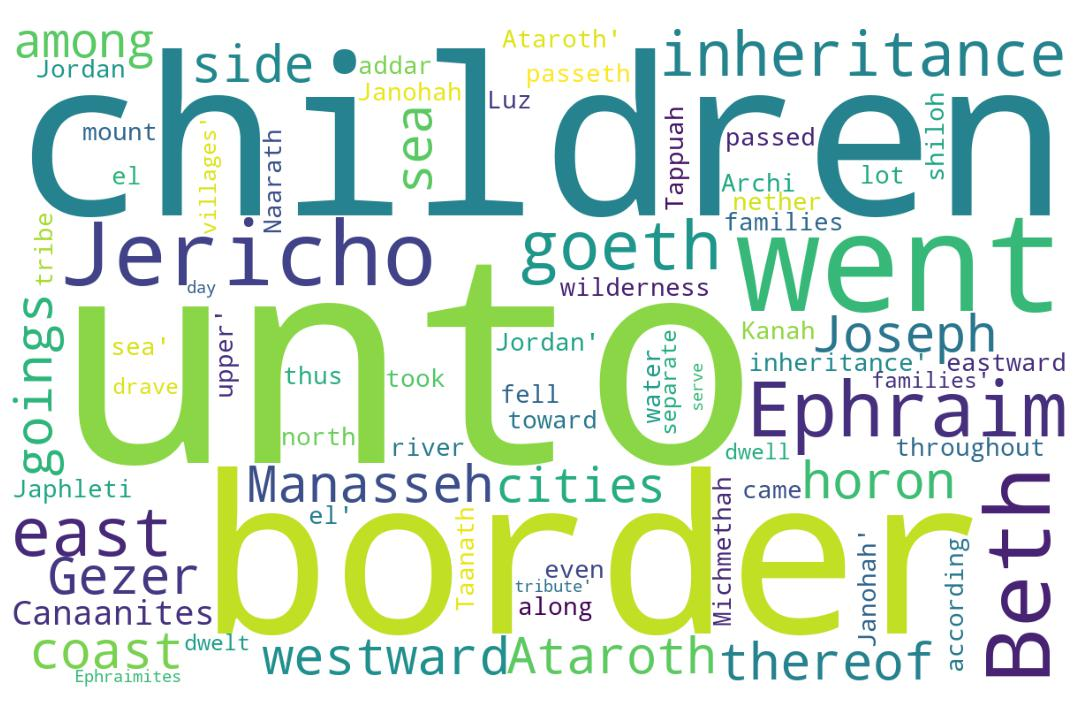
\includegraphics[width=\linewidth]{06OT-Joshua/Joshua16-WordCloud.jpg}
  \caption{Joshua 16 Word Cloud}
  \label{fig:Joshua 16 Word Cloud}
\end{figure}


\marginpar{\scriptsize \centering \fcolorbox{bone}{lime}{\textbf{LAND FOR THE SONS OF JOSEPH}}\\ (Joshua 16:1-10) \begin{compactenum}[I.][8]
	\item The \textbf{Sons}  \index[scripture]{Joshua!Jsh 16:01}  (Jsh 16:1) 
	\item \textbf{Sides of the Compass}  \index[scripture]{Joshua!Jsh 16:02--03}  (Jsh 16:2--3) 
	\item \textbf{Shiloh}  \index[scripture]{Joshua!Jsh 16:06}  (Jsh 16:6) 
	\item The \textbf{Sea} as a Border \index[scripture]{Joshua!Jsh 16:08}  (Jsh 16:8) 
	\item The \textbf{Separate Cities}  \index[scripture]{Joshua!Jsh 16:09}  (Jsh 16:9) 
	\item \textbf{Squatters}  \index[scripture]{Joshua!Jsh 16:10}  (Jsh 16:10) 
	\item Like \textbf{Sin}  \index[scripture]{Joshua!Jsh 16:10}  (Jsh 16:10) 
\end{compactenum}}



\footnote{\textcolor[cmyk]{0.99998,1,0,0}{\hyperlink{TOC}{Return to end of Table of Contents.}}}\footnote{\href{https://audiobible.com/bible/joshua_16.html}{\textcolor[cmyk]{0.99998,1,0,0}{Joshua 16 Audio}}}\textcolor[cmyk]{0.99998,1,0,0}{And the lot of the \fcolorbox{bone}{lime}{children of Joseph} fell from Jordan by Jericho, unto the water of Jericho on the east, to the wilderness that goeth up from Jericho throughout mount Beth-el,} 
[2] \textcolor[cmyk]{0.99998,1,0,0}{And goeth out from Beth-el to Luz, and passeth along unto the borders of Archi to Ataroth,} 
[3] \textcolor[cmyk]{0.99998,1,0,0}{And goeth down westward to the coast of Japhleti, unto the coast of Beth-horon the nether, and to Gezer: and the goings out thereof are at the sea.}
[4] \textcolor[cmyk]{0.99998,1,0,0}{So the children of Joseph, Manasseh and Ephraim, took their inheritance.}\\
\\
\P \textcolor[cmyk]{0.99998,1,0,0}{And the border of the children of Ephraim according to their families was \emph{thus}: even the border of their inheritance on the east side was Ataroth-addar, unto Beth-horon the upper;}
[6] \textcolor[cmyk]{0.99998,1,0,0}{And the border went out toward the sea to Michmethah on the north side; and the border went about eastward unto \fcolorbox{bone}{lime}{Taanath-shiloh}, and passed by it on the east to Janohah;} 
[7] \textcolor[cmyk]{0.99998,1,0,0}{And it went down from Janohah to Ataroth, and to Naarath, and came to Jericho, and went out at Jordan.}
[8] \textcolor[cmyk]{0.99998,1,0,0}{The border went out from Tappuah westward unto the river Kanah; and the goings out thereof were at the \fcolorbox{bone}{lime}{sea}. This \emph{is} the inheritance of the tribe of the children of Ephraim by their families.}
[9] \textcolor[cmyk]{0.99998,1,0,0}{And the \fcolorbox{bone}{lime}{separate cities} for the children of Ephraim \emph{were} among the inheritance of the children of Manasseh, all the cities with their villages.} 
[10] \textcolor[cmyk]{0.99998,1,0,0}{And they drave not out the Canaanites that dwelt in Gezer: but the \fcolorbox{bone}{lime}{Canaanites dwell} among the Ephraimites unto this day, and serve under tribute.} 

\chapter{Joshua 17}

\begin{figure}
  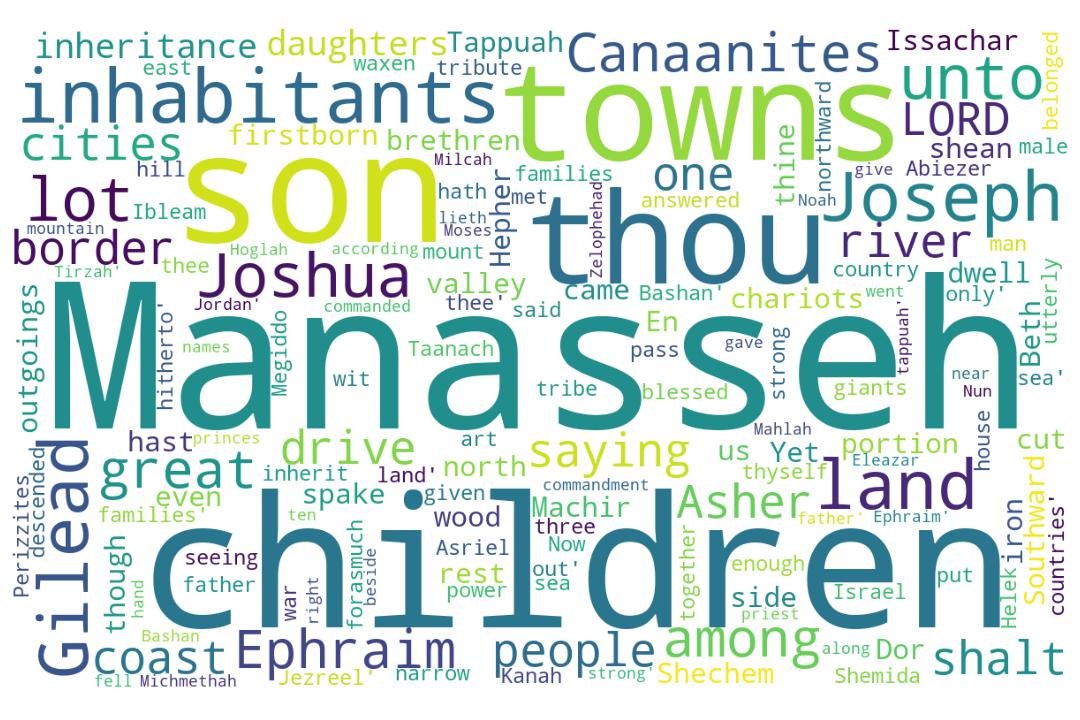
\includegraphics[width=\linewidth]{06OT-Joshua/Joshua17-WordCloud.jpg}
  \caption{Joshua 17 Word Cloud}
  \label{fig:Joshua 17 Word Cloud}
\end{figure}

\marginpar{\scriptsize \centering \fcolorbox{bone}{lime}{\textbf{MANASSEH ON THE WEST SIDE}}\\ (Joshua 17:1-18) \begin{compactenum}[I.][8]
	\item The \textbf{Daughters}  \index[scripture]{Joshua!Jsh 16:03}\index[scripture]{Joshua!Jsh 17:06}  (Jsh 17:3, 6) 
	\item The \textbf{Decree}  \index[scripture]{Joshua!Jsh 16:04}  (Joshua 17:4) (so what happens when the male line to the throne is cut off? This decree determines that Mary's descendant has a right to the throne
	\item The \textbf{Descendants} (the word ``children'' found 13 times in the chapter\index[scripture]{Joshua!Jsh 16:02}  \index[scripture]{Joshua!Jsh 17:08}  \index[scripture]{Joshua!Jsh 17:13}  \index[scripture]{Joshua!Jsh 17:14}  \index[scripture]{Joshua!Jsh 17:16}  (Jsh 17:2 (8x), 8, 12, 13, 14, 16) 
	\item The \textbf{Dwellers}  \index[scripture]{Joshua!Jsh 17:12}\index[scripture]{Joshua!Jsh 17:16}   (Joshua Jsh:12, 16) 
	\item \textbf{Drive} out the Canaanites \index[scripture]{Joshua!Jsh 17:12}\index[scripture]{Joshua!Jsh 17:13} \index[scripture]{Joshua!Jsh 17:18}  (Jsh 17:12, 13, 18) 
	\item We're \textbf{Disdavantaged}  \index[scripture]{Joshua!Jsh 17:12}\index[scripture]{Joshua!Jsh 17:16}   (Jsh 17:16) 
	\item Joshua's \textbf{Determination}  \index[scripture]{Joshua!Jsh 17:18} (Jsh 17:18) 
\end{compactenum}}






\footnote{\textcolor[cmyk]{0.99998,1,0,0}{\hyperlink{TOC}{Return to end of Table of Contents.}}}\footnote{\href{https://audiobible.com/bible/joshua_17.html}{\textcolor[cmyk]{0.99998,1,0,0}{Joshua 17 Audio}}}\textcolor[cmyk]{0.99998,1,0,0}{There was also a lot for the tribe of Manasseh; for he \emph{was} the firstborn of Joseph; \emph{to} \emph{wit}, for Machir the firstborn of Manasseh, the father of Gilead: because he was a man of war, therefore he had Gilead and Bashan.}
[2] \textcolor[cmyk]{0.99998,1,0,0}{There was also \emph{a} \emph{lot} for the rest of the \fcolorbox{bone}{bone}{children of} Manasseh by their families; for the \fcolorbox{bone}{bone}{children of} Abiezer, and for the \fcolorbox{bone}{bone}{children of} Helek, and for the \fcolorbox{bone}{bone}{children of} Asriel, and for the \fcolorbox{bone}{bone}{children of} Shechem, and for the \fcolorbox{bone}{bone}{children of} Hepher, and for the \fcolorbox{bone}{bone}{children of} Shemida: these \emph{were} the male \fcolorbox{bone}{bone}{children of} Manasseh the son of Joseph by their families.}\\
\\
\P \textcolor[cmyk]{0.99998,1,0,0}{But Zelophehad, the son of Hepher, the son of Gilead, the son of Machir, the son of Manasseh, had no sons, but daughters: and these \emph{are} the names of his daughters, \fcolorbox{bone}{lime}{Mahlah}, and \fcolorbox{bone}{lime}{Noah}, \fcolorbox{bone}{lime}{Hoglah}, \fcolorbox{bone}{lime}{Milcah}, and \fcolorbox{bone}{lime}{Trzah}.}
[4] \textcolor[cmyk]{0.99998,1,0,0}{And they came near before Eleazar the priest, and before Joshua the son of Nun, and before the princes, saying, The LORD commanded Moses to give us an inheritance among our brethren. Therefore according to the \fcolorbox{bone}{lime}{commandment} of the LORD he gave them an inheritance among the brethren of their father.}
[5] \textcolor[cmyk]{0.99998,1,0,0}{And there fell ten portions to Manasseh, beside the land of Gilead and Bashan, which \emph{were} on the other side Jordan;}
[6] \textcolor[cmyk]{0.99998,1,0,0}{Because the daughters of Manasseh had an inheritance among his sons: and the rest of Manasseh's sons had the land of Gilead.}\\
\\
\P \textcolor[cmyk]{0.99998,1,0,0}{And the coast of Manasseh was from Asher to Michmethah, that \emph{lieth} before Shechem; and the border went along on the right hand unto the inhabitants of En-tappuah.}
[8] \textcolor[cmyk]{0.99998,1,0,0}{\emph{Now} Manasseh had the land of Tappuah: but Tappuah on the border of Manasseh \emph{belonged} to the \fcolorbox{bone}{bone}{children of} Ephraim;}
[9] \textcolor[cmyk]{0.99998,1,0,0}{And the coast descended unto the river Kanah, southward of the river: these cities of Ephraim \emph{are} among the cities of Manasseh: the coast of Manasseh also \emph{was} on the north side of the river, and the outgoings of it were at the sea:}
[10] \textcolor[cmyk]{0.99998,1,0,0}{Southward \emph{it} \emph{was} Ephraim's, and northward \emph{it} \emph{was} Manasseh's, and the sea is his border; and they met together in Asher on the north, and in Issachar on the east.}
[11] \textcolor[cmyk]{0.99998,1,0,0}{And Manasseh had in Issachar and in Asher Beth-shean and her towns, and Ibleam and her towns, and the inhabitants of Dor and her towns, and the inhabitants of En-dor and her towns, and the inhabitants of Taanach and her towns, and the inhabitants of Megiddo and her towns, \emph{even} three countries.}
[12] \textcolor[cmyk]{0.99998,1,0,0}{Yet the \fcolorbox{bone}{bone}{children of} Manasseh could not \fcolorbox{bone}{lime}{drive out} \emph{the} \emph{inhabitants} \emph{of} those cities; but the Canaanites would \fcolorbox{bone}{lime}{dwell} in that land.}
[13] \textcolor[cmyk]{0.99998,1,0,0}{Yet it came to pass, when the \fcolorbox{bone}{bone}{children of} Israel were waxen strong, that they put the Canaanites to tribute; but did not utterly drive them out.}
[14] \textcolor[cmyk]{0.99998,1,0,0}{And the \fcolorbox{bone}{bone}{children of} Joseph spake unto Joshua, saying, Why hast thou given me \emph{but} one lot and one portion to inherit, seeing I \emph{am} a great people, forasmuch as the LORD hath blessed me hitherto?}
[15] \textcolor[cmyk]{0.99998,1,0,0}{And Joshua answered them, If thou \emph{be} a great people, \emph{then} get thee up to the wood \emph{country}, and cut down for thyself there in the land of the Perizzites and of the giants, if mount Ephraim be too narrow for thee.}
[16] \textcolor[cmyk]{0.99998,1,0,0}{And the \fcolorbox{bone}{bone}{children of} Joseph said, The hill is \fcolorbox{bone}{lime}{not enough} for us: and all the Canaanites that dwell in the land of the valley have chariots of iron, \emph{both} \emph{they} who \emph{are} of Beth-shean and her towns, and \emph{they} who \emph{are} of the valley of Jezreel.}
[17] \textcolor[cmyk]{0.99998,1,0,0}{And Joshua spake unto the house of Joseph, \emph{even} to Ephraim and to Manasseh, saying, Thou \emph{art} a great people, and hast great power: thou shalt not have one lot \emph{only}:}
[18] \textcolor[cmyk]{0.99998,1,0,0}{But the mountain shall be thine; for it \emph{is} a wood, and thou shalt cut it down: and the outgoings of it shall be thine: for \fcolorbox{bone}{lime}{thou shalt} drive out the Canaanites, though they have iron chariots, \emph{and} though they \emph{be} strong.}
\chapter{Joshua 18}

\begin{figure}
  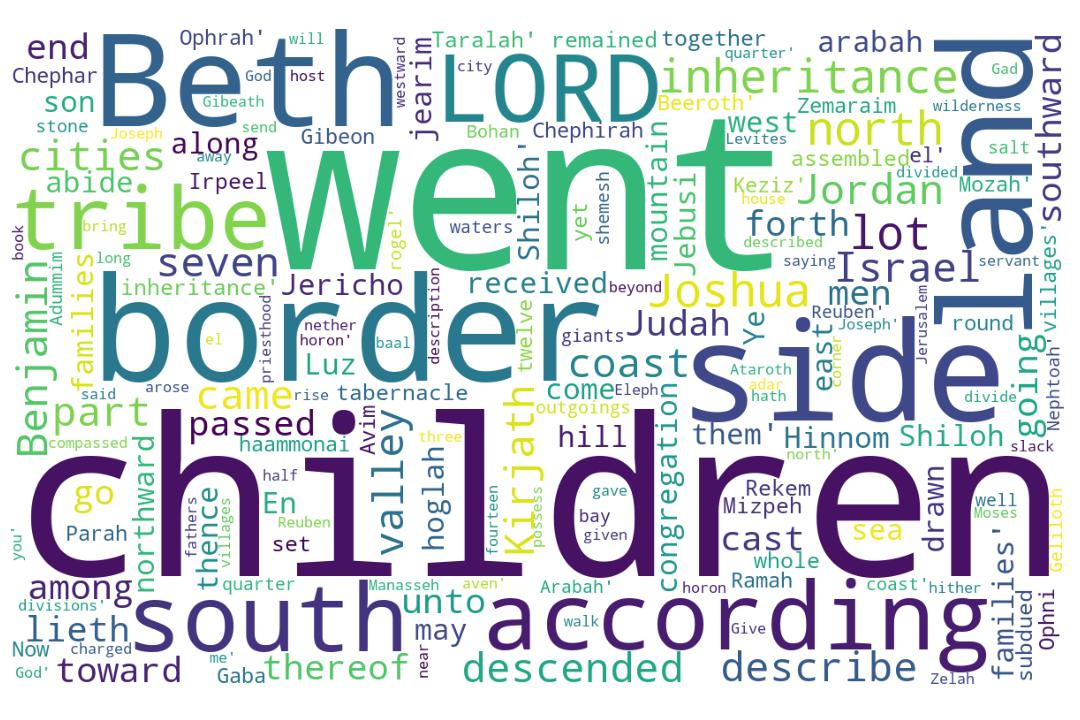
\includegraphics[width=\linewidth]{06OT-Joshua/Joshua18-WordCloud.jpg}
  \caption{Joshua 18 Word Cloud}
  \label{fig:Joshua 18 Word Cloud}
\end{figure}


\marginpar{\scriptsize \centering \fcolorbox{bone}{lime}{\textbf{LAND FOR BENJAMIN}}\\ (Joshua 18:1-28) \begin{compactenum}[I.][8]
	\item A Land \textbf{Subdued}  \index[scripture]{Joshua!Jsh 18:01} (Jsh 18:1) 
	\item A \textbf{Slackness}  \index[scripture]{Joshua!Jsh 18:03} (Jsh 18:3) 
	\item The \textbf{Scouts}  \index[scripture]{Joshua!Jsh 18:04} (Jsh 18:4) 
	\item  \textbf{Seven} Portions \index[scripture]{Joshua!Jsh 18:05} (Jsh 18:5) 
	\item The \textbf{Specfics}  \index[scripture]{Joshua!Jsh 18:11--28} (Jsh 18:11--28) 
	\item A Solid \textbf{Strategy} for Decisions -- analysis, counsel, prayer % \index[scripture]{Joshua!Jsh 18:11--28} (Jsh 18:11--28) 
\end{compactenum}}


\footnote{\textcolor[cmyk]{0.99998,1,0,0}{\hyperlink{TOC}{Return to end of Table of Contents.}}}\footnote{\href{https://audiobible.com/bible/joshua_18.html}{\textcolor[cmyk]{0.99998,1,0,0}{Joshua 18 Audio}}}\textcolor[cmyk]{0.99998,1,0,0}{And the whole congregation of the children of Israel assembled together at Shiloh, and set up the tabernacle of the congregation there. And the land was \fcolorbox{bone}{lime}{subdued} before them.}
[2] \textcolor[cmyk]{0.99998,1,0,0}{And there remained among the children of Israel seven tribes, which had not yet received their inheritance.}
[3] \textcolor[cmyk]{0.99998,1,0,0}{And Joshua said unto the children of Israel, How long \emph{are} ye \fcolorbox{bone}{lime}{slack} to go to possess the land, which the LORD God of your fathers hath given you?}
[4] \textcolor[cmyk]{0.99998,1,0,0}{Give out from among you three men for \emph{each} tribe: and I will send them, and they shall rise, and go \fcolorbox{bone}{lime}{through the land}, and describe it according to the inheritance of them; and they shall come \emph{again} to me.}
[5] \textcolor[cmyk]{0.99998,1,0,0}{And they shall divide it into \fcolorbox{bone}{lime}{seven parts}: Judah shall abide in their coast on the south, and the house of Joseph shall abide in their coasts on the north.}
[6] \textcolor[cmyk]{0.99998,1,0,0}{Ye shall therefore describe the land \emph{into} seven parts, and bring \emph{the} \emph{description} hither to me, that I may cast lots for you here before the LORD our God.}
[7] \textcolor[cmyk]{0.99998,1,0,0}{But the Levites have no part among you; for the priesthood of the LORD \emph{is} their inheritance: and Gad, and Reuben, and half the tribe of Manasseh, have received their inheritance beyond Jordan on the east, which Moses the servant of the LORD gave them.}\\
\\
\P \textcolor[cmyk]{0.99998,1,0,0}{And the men arose, and went away: and Joshua charged them that went to describe the land, saying, Go and walk through the land, and describe it, and come again to me, that I may here cast lots for you before the LORD in Shiloh.}
[9] \textcolor[cmyk]{0.99998,1,0,0}{And the men went and passed through the land, and described it by cities into seven parts in a book, and came \emph{again} to Joshua to the host at Shiloh.}\\
\\
\P \textcolor[cmyk]{0.99998,1,0,0}{And Joshua cast lots for them in Shiloh before the LORD: and there Joshua divided the land unto the children of Israel according to their divisions.}\\
\\
\P \textcolor[cmyk]{0.99998,1,0,0}{And \fcolorbox{bone}{lime}{the lot} of the tribe of the children of Benjamin came up according to their families: and the coast of their lot came forth between the children of Judah and the children of Joseph.}
[12] \textcolor[cmyk]{0.99998,1,0,0}{And their border on the north side was from Jordan; and the border went up to the side of Jericho on the north side, and went up through the mountains westward; and the goings out thereof were at the wilderness of Beth-aven.}
[13] \textcolor[cmyk]{0.99998,1,0,0}{And the border went over from thence toward Luz, to the side of Luz, which \emph{is} Beth-el, southward; and the border descended to Ataroth-adar, near the hill that \emph{lieth} on the south side of the nether Beth-horon.}
[14] \textcolor[cmyk]{0.99998,1,0,0}{And the border was drawn \emph{thence}, and compassed the corner of the sea southward, from the hill that \emph{lieth} before Beth-horon southward; and the goings out thereof were at Kirjath-baal, which \emph{is} Kirjath-jearim, a city of the children of Judah: this \emph{was} the west quarter.}
[15] \textcolor[cmyk]{0.99998,1,0,0}{And the south quarter \emph{was} from the end of Kirjath-jearim, and the border went out on the west, and went out to the well of waters of Nephtoah:}
[16] \textcolor[cmyk]{0.99998,1,0,0}{And the border came down to the end of the mountain that \emph{lieth} before the valley of the son of Hinnom, \emph{and} which \emph{is} in the valley of the giants on the north, and descended to the valley of Hinnom, to the side of Jebusi on the south, and descended to En-rogel,}
[17] \textcolor[cmyk]{0.99998,1,0,0}{And was drawn from the north, and went forth to En-shemesh, and went forth toward Geliloth, which \emph{is} over against the going up of Adummim, and descended to the stone of Bohan the son of Reuben,}
[18] \textcolor[cmyk]{0.99998,1,0,0}{And passed along toward the side over against Arabah northward, and went down unto Arabah:}
[19] \textcolor[cmyk]{0.99998,1,0,0}{And the border passed along to the side of Beth-hoglah northward: and the outgoings of the border were at the north bay of the salt sea at the south end of Jordan: this \emph{was} the south coast.}
[20] \textcolor[cmyk]{0.99998,1,0,0}{And Jordan was the border of it on the east side. This \emph{was} the inheritance of the children of Benjamin, by the coasts thereof round about, according to their families.}
[21] \textcolor[cmyk]{0.99998,1,0,0}{Now the cities of the tribe of the children of Benjamin according to their families were Jericho, and Beth-hoglah, and the valley of Keziz,}
[22] \textcolor[cmyk]{0.99998,1,0,0}{And Beth-arabah, and Zemaraim, and Beth-el,}
[23] \textcolor[cmyk]{0.99998,1,0,0}{And Avim, and Parah, and Ophrah,}
[24] \textcolor[cmyk]{0.99998,1,0,0}{And Chephar-haammonai, and Ophni, and Gaba; twelve cities with their villages:}
[25] \textcolor[cmyk]{0.99998,1,0,0}{Gibeon, and Ramah, and Beeroth,}
[26] \textcolor[cmyk]{0.99998,1,0,0}{And Mizpeh, and Chephirah, and Mozah,}
[27] \textcolor[cmyk]{0.99998,1,0,0}{And Rekem, and Irpeel, and Taralah,}
[28] \textcolor[cmyk]{0.99998,1,0,0}{And Zelah, Eleph, and Jebusi, which \emph{is} Jerusalem, Gibeath, \emph{and} Kirjath; fourteen cities with their villages. This \emph{is} the inheritance of the children of Benjamin according to their families.}


\chapter{Psalm 70}

\begin{figure}
  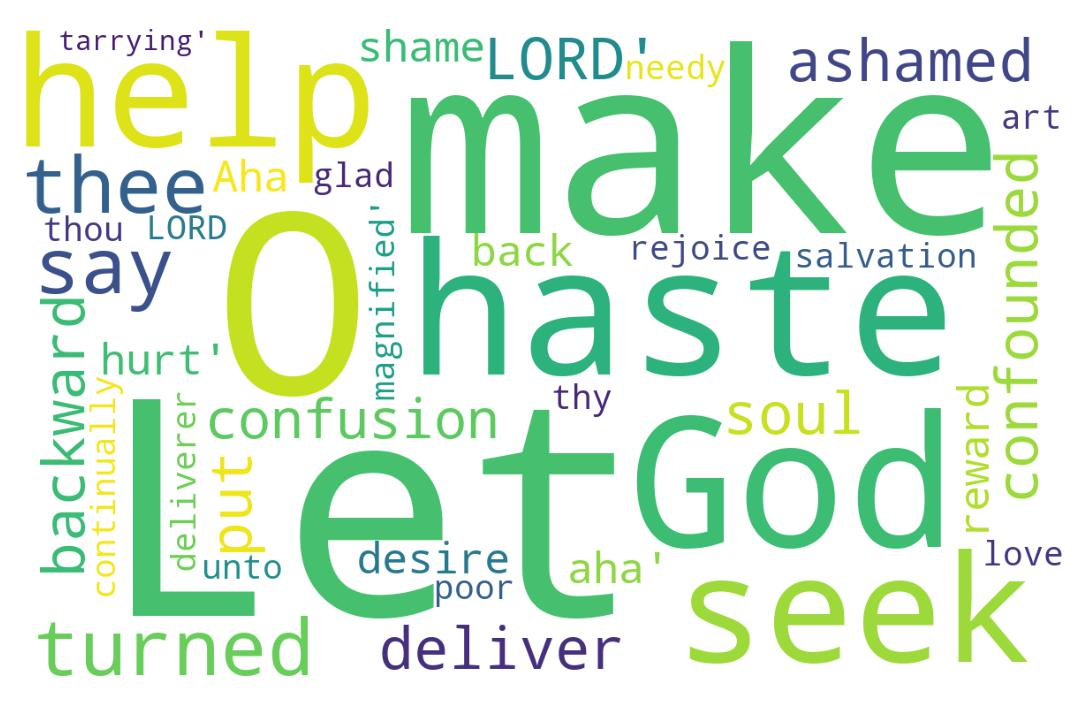
\includegraphics[width=\linewidth]{19OT-Psalms/Psalm70-WordCloud.jpg}
  \caption{Psalm 70 Word Cloud}
  \label{fig:Psalm 70 word Cloud}
\end{figure}



% \textcolor[cmyk]{0.99998,1,0,0}{
\marginpar{\scriptsize \centering \fcolorbox{bone}{lime}{\textbf{DAVID'S EMERGENCY PRAYER}}\\ (Psalm 70) \begin{compactenum}[I.][8]

     \item The \textbf{Distress} \index[scripture]{Psalms!Psa 070:01}(Psa 70:1)
    \item David's \textbf{Determination} \index[scripture]{Psalms!Psa 070:01}(Psa 70:1)
    \item The \textbf{Desire} of the Wicked\index[scripture]{Psalms!Psa 070:02}(Psa 70:2)
    \item Two \textbf{Different} Groups of People \index[scripture]{Psalms!Psa 070:03}\index[scripture]{Psalms!Psa 070:04}(Psa 70:3, 4)
    \item A \textbf{Declaration} \index[scripture]{Psalms!Psa 070:04}(Psa 70:4)
    \item The \textbf{Deliverer} \index[scripture]{Psalms!Psa 070:05}(Psa 70:5)
    \item A \textbf{Dependence} \index[scripture]{Psalms!Psa 070:05}(Psa 70:5)
\end{compactenum}}




\footnote{\textcolor[rgb]{0.00,0.25,0.00}{\hyperlink{TOC}{Return to end of Table of Contents.}}}\footnote{\href{https://audiobible.com/bible/psalms_70.html}{\textcolor[cmyk]{0.99998,1,0,0}{Psalm 70 Audio}}}\textcolor[cmyk]{0.99998,1,0,0}{To the chief Musician, \emph{A Psalm} of David, to bring to remembrance.}\\
\\
\textcolor[cmyk]{0.99998,1,0,0}{\emph{Make} \emph{haste}, O God, to deliver me; make haste to help me, O LORD.}
[2] \textcolor[cmyk]{0.99998,1,0,0}{Let them be ashamed and confounded that seek after my soul: let them be turned backward, and put to confusion, that desire my hurt.}
[3] \textcolor[cmyk]{0.99998,1,0,0}{Let them be turned back for a reward of their shame that say, Aha, aha.}
[4] \textcolor[cmyk]{0.99998,1,0,0}{Let all those that seek thee rejoice and be glad in thee: and let such as love thy salvation say continually, Let God be magnified.}
[5] \textcolor[cmyk]{0.99998,1,0,0}{But I \emph{am} poor and needy: make haste unto me, O God: thou \emph{art} my help and my deliverer; O LORD, make no tarrying.}








\chapter{Proverb 11}

\begin{figure}
  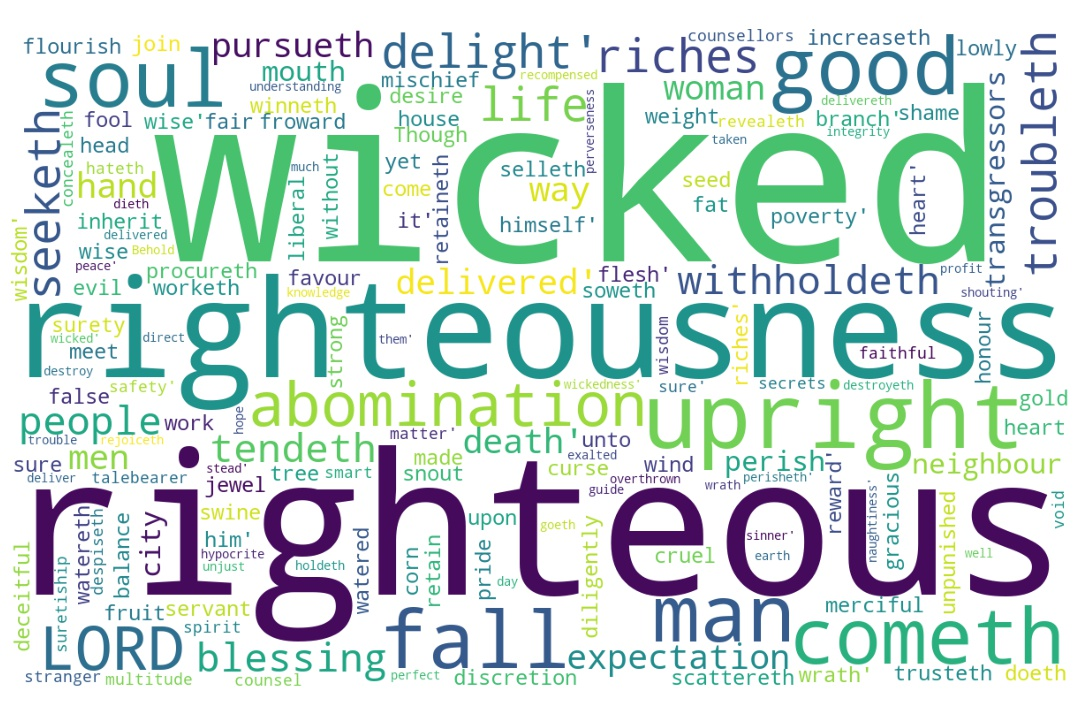
\includegraphics[width=\linewidth]{20OT-Proverbs/Proverb11-WordCloud.jpg}
  \caption{Proverb 11 Word Cloud}
  \label{fig:Proverb 11 Word Cloud}
\end{figure}

\marginpar{\scriptsize \centering \fcolorbox{bone}{lime}{\textbf{MISSING IMPORTANT THINGS}}\\ (Proverbs 11:1-31) \begin{compactenum}[I.][8]
    \item No \textbf{Balance} \index[scripture]{Proverbs!Pro 11:01} (Pro 11:1) 
    \item No \textbf{Integrity} \index[scripture]{Proverbs!Pro 11:03}(Pro 11:3) 
    \item No \textbf{Expectation} \index[scripture]{Proverbs!Pro 11:07}(Pro 11:7) 
    \item No \textbf{Wisdom} \index[scripture]{Proverbs!Pro 11:12}(Pro 11:12) 
    \item No \textbf{Counsel} \index[scripture]{Proverbs!Pro 11:14}(Pro 11:14) 
    \item No \textbf{Discretion} \index[scripture]{Proverbs!Pro 11:22}(Pro 11:22) 
    \item No \textbf{Corn (food)} \index[scripture]{Proverbs!Pro 11:26}(Pro 11:26) 
\end{compactenum}}

\marginpar{\scriptsize \centering \fcolorbox{bone}{yellow}{\textbf{UNDEPENDABLE}}\\ (Proverbs 11:1-31) \begin{compactenum}[I.][8]
    \item \textbf{Riches in the Day of Wrath} \index[scripture]{Proverbs!Pro 11:04}\index[scripture]{Proverbs!Pro 11:28}(Pro 11:4, 28)
    \item \textbf{A Hypocrite to Keep his Word} \index[scripture]{Proverbs!Pro 11:09}(Pro 11:9)
    \item \textbf{Mouth of the Wicked}\index[scripture]{Proverbs!Pro 11:11} (Pro 11:11)
    \item \textbf{A Foolish Neighbor Providing Wisdom} \index[scripture]{Proverbs!Pro 11:12}(Pro 11:12)
    \item \textbf{Lasting Blessing from a Deceitful Work} \index[scripture]{Proverbs!Pro 11:18}(Pro 11:18)
    \item \textbf{Discretion from an Evil Woman} \index[scripture]{Proverbs!Pro 11:22} (Pro 11:22)
    \item \textbf{A Fool to not Withhold}\index[scripture]{Proverbs!Pro 11:24}\index[scripture]{Proverbs!Pro 11:27} (Pro 11:24, 27)
\end{compactenum}}

\marginpar{\scriptsize \centering \fcolorbox{bone}{black}{\textbf{\textcolor[cmyk]{0,0,0,0}{WALKING THE RIGHT PATH}}}\\ (Proverbs 11) \begin{compactenum}[I.][8]
    \item The \textbf{Delight of the Lord} \index[scripture]{Proverbs!Pro 11:01}\index[scripture]{Proverbs!Pro 11:20}(Pro 11:1, 20)
     \item   \textbf{Deliverance} \index[scripture]{Proverbs!Pro 11:04}  \index[scripture]{Proverbs!Pro 11:06} \index[scripture]{Proverbs!Pro 11:08} \index[scripture]{Proverbs!Pro 11:09} \index[scripture]{Proverbs!Pro 11:21}(Pro 11:4, 6, 8, 9, 21)
     \item  A \textbf{Directing} \index[scripture]{Proverbs!Pro 11:05} (Pro 11:5)
   \item  \textbf{Discretion} \index[scripture]{Proverbs!Pro 11:22} (Pro 11:22)
   \item  \textbf{Desire} \index[scripture]{Proverbs!Pro 11:23} (Pro 11:23)
   \item  \textbf{Diligence} \index[scripture]{Proverbs!Pro 11:27} (Pro 11:27)
    \item  A \textbf{Destination} \index[scripture]{Proverbs!Pro 11:30} (Pro 11:30)
\end{compactenum}}

\marginpar{\scriptsize \centering 
\fcolorbox{black}{blue}{\textbf{\textcolor[cmyk]{0,0,0,0}{A PERSON OUT OF BALANCE}}}\\ 
(Proverbs 11:1) 
\begin{compactenum}[I.][8]
    \item \textbf{Tends to Fall a Lot}  
    \item \textbf{Breaks Things}
    \item \textbf{Bumps Into Things}  
    \item \textbf{Looks Funny or Foolish or Pathetic}
    \item \textbf{Usually Needs a Crutch}
    \item \textbf{Requires Extra Attention}
    \item \textbf{Throws off Judgment}
\end{compactenum}}




\footnote{\textcolor[cmyk]{0.99998,1,0,0}{\hyperlink{TOC}{Return to end of Table of Contents.}}}\footnote{\href{https://www.audioverse.org/english/audiobibles/books/ENGKJV/O/Prov/1}{\textcolor[cmyk]{0.99998,1,0,0}{Proverbs Audio}}}\textcolor[cmyk]{0.99998,1,0,0}{A \fcolorbox{bone}{lime}{false balance} \emph{is} abomination to the LORD: but \fcolorbox{bone}{bone}{a} just weight \emph{is} \fcolorbox{bone}{bone}{his} delight.}\footnote{\textbf{Proverb 16:11} - A just weight and balance are the LORD's: all the weights of the bag are his work.}\footnote{\textbf{Proverb 20:10} - Divers weights, and divers measures, both of them are alike abomination to the LORD.}\footnote{\textbf{Proverb 20:23} - Divers weights are an abomination unto the LORD; and a false balance is not good.}\footnote{\textbf{Ezekiel 45:10-12} - Ye shall have just balances, and a just ephah, and a just bath. [11] The ephah and the bath shall be of one measure, that the bath may contain the tenth part of an homer, and the ephah the tenth part of an homer: the measure thereof shall be after the homer. [12] And the shekel shall be twenty gerahs: twenty shekels, five and twenty shekels, fifteen shekels, shall be your maneh.}\footnote{\textbf{Hosea 12:7} - He is a merchant, the balances of deceit are in his hand: he loveth to oppress.}\footnote{\textbf{Amos 8:5-6} - Saying, When will the new moon be gone, that we may sell corn? and the sabbath, that we may set forth wheat, making the ephah small, and the shekel great, and falsifying the balances by deceit? That we may buy the poor for silver, and the needy for a pair of shoes; yea, and sell the refuse of the wheat?}\footnote{\textbf{Micah 6:10-11} - Are there yet the treasures of wickedness in the house of the wicked, and the scant measure that is abominable? Shall I count them pure with the wicked balances, and with the bag of deceitful weights?}
[2] \textcolor[cmyk]{0.99998,1,0,0}{\emph{When} pride cometh, then cometh shame: but with the lowly \emph{is} wisdom.}\footnote{\textbf{Proverb 16:18-19} - Pride goeth before destruction, and an haughty spirit before a fall. [19] Better it is to be of an humble spirit with the lowly, than to divide the spoil with the proud.}\footnote{\textbf{Daniel 4:30-32} - The king spake, and said, Is not this great Babylon, that I have built for the house of the kingdom by the might of my power, and for the honour of my majesty? [31] While the word was in the king's mouth, there fell a voice from heaven, saying, O king Nebuchadnezzar, to thee it is spoken; The kingdom is departed from thee. [32] And they shall drive thee from men, and thy dwelling shall be with the beasts of the field: they shall make thee to eat grass as oxen, and seven times shall pass over thee, until thou know that the most High ruleth in the kingdom of men, and giveth it to whomsoever he will.}\footnote{\textbf{Proverb 15:33} - The fear of the LORD is the instruction of wisdom; and before honour is humility.}\footnote{\textbf{1 Corinthians 8:1-2} - Now as touching things offered unto idols, we know that we all have knowledge. Knowledge puffeth up, but charity edifieth. [2] And if any man think that he knoweth any thing, he knoweth nothing yet as he ought to know.}
[3] \textcolor[cmyk]{0.99998,1,0,0}{The \fcolorbox{bone}{lime}{integrity} of the upright shall guide them: but the perverseness of \fcolorbox{bone}{MYGOLD}{transgressors} shall destroy them.}
[4] \textcolor[cmyk]{0.99998,1,0,0}{Riches profit not in the day of wrath: but \fcolorbox{bone}{MYGOLD}{righteousness} delivereth from death.}
[5] \textcolor[cmyk]{0.99998,1,0,0}{The \fcolorbox{bone}{MYGOLD}{righteousness} of the perfect shall direct \fcolorbox{bone}{bone}{his} way: but the wicked shall fall by \fcolorbox{bone}{bone}{his} own wickedness.}
[6] \textcolor[cmyk]{0.99998,1,0,0}{The \fcolorbox{bone}{MYGOLD}{righteousness} of the upright shall deliver them: but \fcolorbox{bone}{MYGOLD}{transgressors} shall be taken in \emph{their} \emph{own} naughtiness.}
[7] \textcolor[cmyk]{0.99998,1,0,0}{When \fcolorbox{bone}{bone}{a} wicked man dieth, \emph{his} \fcolorbox{bone}{lime}{expectation} shall perish: and the hope of unjust \emph{men} perisheth.}
[8] \textcolor[cmyk]{0.99998,1,0,0}{The righteous is delivered out of trouble, and the wicked cometh in \fcolorbox{bone}{bone}{his} stead.}
[9] \textcolor[cmyk]{0.99998,1,0,0}{An hypocrite with \emph{his} mouth destroyeth \fcolorbox{bone}{bone}{his} neighbour: but through knowledge shall the just be delivered.}
[10] \textcolor[cmyk]{0.99998,1,0,0}{When it goeth well with the righteous, the city rejoiceth: and when the wicked perish, \emph{there} \emph{is} shouting.}
[11] \textcolor[cmyk]{0.99998,1,0,0}{By the blessing of the upright the city is exalted: but it is overthrown by the mouth of the wicked.}
[12] \textcolor[cmyk]{0.99998,1,0,0}{He that is void of \fcolorbox{bone}{lime}{wisdom} despiseth \fcolorbox{bone}{bone}{his} neighbour: but \fcolorbox{bone}{bone}{a} man of \fcolorbox{bone}{MYGOLD}{understanding} holdeth \fcolorbox{bone}{bone}{his} peace.}
[13] \textcolor[cmyk]{0.99998,1,0,0}{A talebearer revealeth secrets: but he that is of \fcolorbox{bone}{bone}{a} faithful spirit concealeth the matter.}
[14] \textcolor[cmyk]{0.99998,1,0,0}{Where \fcolorbox{bone}{lime}{no counsel} \emph{is}, the people fall: but in the multitude of counsellors \emph{there} \emph{is} safety.}\footnote{\textbf{Proverb 15:22} - Without counsel purposes are disappointed: but in the multitude of counsellors they are established.}\footnote{\textbf{Proverb 16:22} - Understanding is a wellspring of life unto him that hath it: but the instruction of fools is folly.}\footnote{\textbf{Proverb 24:6} - For by wise counsel thou shalt make thy war: and in multitude of counsellors there is safety.}
[15] \textcolor[cmyk]{0.99998,1,0,0}{He that is surety for \fcolorbox{bone}{bone}{a} stranger shall smart \emph{for} \emph{it}: and he that hateth suretiship is sure.}\footnote{\textbf{Proverb 6:1-5} - My son, if thou be surety for thy friend, if thou hast stricken thy hand with a stranger, [2] Thou art snared with the words of thy mouth, thou art taken with the words of thy mouth. [3] Do this now, my son, and deliver thyself, when thou art come into the hand of thy friend; go, humble thyself, and make sure thy friend. [4] Give not sleep to thine eyes, nor slumber to thine eyelids. [5] Deliver thyself as a roe from the hand of the hunter, and as a bird from the hand of the fowler.}
[16] \textcolor[cmyk]{0.99998,1,0,0}{A gracious woman retaineth honour: and strong \emph{men} retain riches.}
[17] \textcolor[cmyk]{0.99998,1,0,0}{The merciful man doeth good to \fcolorbox{bone}{bone}{his} own soul: but \emph{he} \emph{that} \emph{is} cruel troubleth \fcolorbox{bone}{bone}{his} own flesh.}
[18] \textcolor[cmyk]{0.99998,1,0,0}{The wicked worketh \fcolorbox{bone}{bone}{a} deceitful work: but to him that soweth \fcolorbox{bone}{MYGOLD}{righteousness} \emph{shall} \emph{be} \fcolorbox{bone}{bone}{a} sure reward.}
[19] \textcolor[cmyk]{0.99998,1,0,0}{As \fcolorbox{bone}{MYGOLD}{righteousness} \emph{tendeth} to life: so he that pursueth evil \emph{pursueth} \emph{it} to \fcolorbox{bone}{bone}{his} own death.}
[20] \textcolor[cmyk]{0.99998,1,0,0}{They that are of \fcolorbox{bone}{bone}{a} froward heart \emph{are} abomination to the LORD: but \emph{such} \emph{as} \emph{are} upright in \emph{their} way \emph{are} \fcolorbox{bone}{bone}{his} delight.}
[21] \textcolor[cmyk]{0.99998,1,0,0}{\emph{Though} hand \emph{join} in hand, the wicked shall not be unpunished: but the seed of the righteous shall be delivered.}
[22] \textcolor[cmyk]{0.99998,1,0,0}{\emph{As} a jewel of gold in \fcolorbox{bone}{bone}{a} swine's snout, \emph{so} \emph{is} \fcolorbox{bone}{bone}{a} fair woman which is without \fcolorbox{bone}{lime}{discretion}.}
[23] \textcolor[cmyk]{0.99998,1,0,0}{The desire of the righteous \emph{is} only good: \emph{but} the expectation of the wicked \emph{is} wrath.}
[24] \textcolor[cmyk]{0.99998,1,0,0}{There is that scattereth, and yet increaseth; and \emph{there} \emph{is} that withholdeth more than is meet, but \emph{it} \emph{tendeth} to poverty.}
[25] \textcolor[cmyk]{0.99998,1,0,0}{The liberal soul shall be made fat: and he that watereth shall be watered also himself.}
[26] \textcolor[cmyk]{0.99998,1,0,0}{He that \fcolorbox{bone}{lime}{withholdeth corn}, the people shall curse him: but blessing \emph{shall} \emph{be} upon the head of him that selleth \emph{it}.}
[27] \textcolor[cmyk]{0.99998,1,0,0}{He that diligently seeketh good procureth favour: but he that seeketh mischief, it shall come unto him.}
[28] \textcolor[cmyk]{0.99998,1,0,0}{He that trusteth in \fcolorbox{bone}{bone}{his} riches shall fall: but the righteous shall flourish as \fcolorbox{bone}{bone}{a} branch.}
[29] \textcolor[cmyk]{0.99998,1,0,0}{He that troubleth \fcolorbox{bone}{bone}{his} own house shall inherit the wind: and the fool \emph{shall} \emph{be} servant to the wise of heart.}\footnote{\textbf{1 Samuel 25:3, 17, 38} - Now the name of the man was Nabal; and the name of his wife Abigail: and she was a woman of good understanding, and of a beautiful countenance: but the man was churlish and evil in his doings; and he was of the house of Caleb. [17] Now therefore know and consider what thou wilt do; for evil is determined against our master, and against all his household: for he is such a son of Belial, that a man cannot speak to him. [38] And it came to pass about ten days after, that the LORD smote Nabal, that he died.}\footnote{\textbf{Hosea 8:7} - For they have sown the wind, and they shall reap the whirlwind: it hath no stalk: the bud shall yield no meal: if so be it yield, the strangers shall swallow it up.}
[30] \textcolor[cmyk]{0.99998,1,0,0}{The fruit of the righteous \emph{is} \fcolorbox{bone}{bone}{a} tree of life; and he that winneth souls \emph{is} wise.}\footnote{\textbf{Proverb 3:18} - She is a tree of life to them that lay hold upon her: and happy is every one that retaineth her.}\footnote{\textbf{Proverb 15:4} -A wholesome tongue is a tree of life: but perverseness therein is a breach in the spirit.}\footnote{\textbf{Daniel 12:3} - And they that be wise shall shine as the brightness of the firmament; and they that turn many to righteousness as the stars for ever and ever.}\footnote{\textbf{James 5:20} - Let him know, that he which converteth the sinner from the error of his way shall save a soul from death, and shall hide a multitude of sins.}
[31] \textcolor[cmyk]{0.99998,1,0,0}{Behold, the righteous shall be recompensed in the earth: much more the wicked and the sinner.}


\end{document}

